\documentclass[withoutpreface,bwprint]{cumcmthesis} %去掉封面与编号页
\title{实验报告-实验三}
\author{18340206张德龙 \\
	zhangdlong3@mail2.sysu.edu.cn
}
\date{\today}
\usepackage[cache=false]{minted}
\usepackage{diagbox}
%\usepackage{fancyhdr}
%\pagestyle{empty} 
{\renewcommand\fcolorbox[4][]{\textcolor{cyan}{\strut#4}} %屏蔽汇编语言mint的错误
\graphicspath{{figure/}}

\let\algorithm\relax  
\let\endalgorithm\relax 
\usepackage[linesnumbered,ruled,lined]{algorithm2e}
\usepackage{algpseudocode}  
\renewcommand{\algorithmicrequire}{\textbf{Input:}}   
\renewcommand{\algorithmicensure}{\textbf{Output:}}   
\SetKwFor{For}{for}{do}{endfor}
\newcommand{\ret}{\textbf{return}}   

\makeatletter
\newenvironment{breakablealgorithm}
{% \begin{breakablealgorithm}
	\begin{center}
		\refstepcounter{algorithm}% New algorithm
		\hrule height.8pt depth0pt \kern2pt% \@fs@pre for \@fs@ruled
		\renewcommand{\caption}[2][\relax]{% Make a new \caption
			{\raggedright\textbf{\ALG@name~\thealgorithm} ##2\par}%
			\ifx\relax##1\relax % #1 is \relax
			\addcontentsline{loa}{algorithm}{\protect\numberline{\thealgorithm}##2}%
			\else % #1 is not \relax
			\addcontentsline{loa}{algorithm}{\protect\numberline{\thealgorithm}##1}%
			\fi
			\kern2pt\hrule\kern2pt
		}
	}{% \end{breakablealgorithm}
		\kern2pt\hrule\relax% \@fs@post for \@fs@ruled
	\end{center}
}
\makeatother

\newcounter{Emp}[subsubsection]	% 设置计数器
\newcommand{\kuohao}{\addtocounter{Emp}{1} \noindent (\theEmp)}

\usepackage{amssymb}% http://ctan.org/pkg/amssymb
\usepackage{pifont}% http://ctan.org/pkg/pifont
\newcommand{\cmark}{\ding{51}}%
\newcommand{\xmark}{\ding{55}}%

\usepackage{threeparttable}

\begin{document}
\maketitle
\begin{abstract}
 
 摘要:简要介绍要解决的问题,所使用的方法步骤,取得的结果或结论。
 \keywords{1 \quad 2 \quad 3}
\end{abstract}

\section{导言}

	
	
	车辆路径规划是现代交通的一项重要任务。优化车辆路线不仅可以
	大大降低运营成本,同时也能够提高客户满意度。然而,车辆路径问题(VRP问题,即Vehicle Routing Problem)为NP难问题,
	在有效解决大规模问题上仍具有十足的挑战性。
	在论文\cite{1}中,作者提出了一种新颖的深度学习模型,其通过将点和边的信息进行嵌入,然后通过结合强化学习和分类任务的方法来学习
	生成车辆路线安排的启发式策略,本实验的目的即为复现其论文中使用的方法和结果。

\section{实验过程}

\subsection{总体结构}
	结合论文\cite{1}中的思想,本次实验我们小组所实现的模型结构示意图如下:
	\begin{figure}[H]
		\centering
		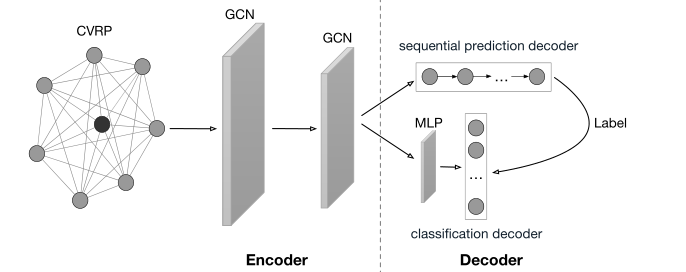
\includegraphics[width=1\linewidth]{struct}
		\caption{模型结构}
	\end{figure}
	本实验中实现的深度模型采用编码-解码(encoder-decoder)架构,其中编码部件将问题中的边和点编码为具有边。点信息的实数嵌入,然后将这些嵌入输入两个联合训练的解码器——序列预测解码器(squential prediction decoder)和分类解码器(classification  decoder)来进行问题的求解。

\subsection{编码器}

	编码器主要通过仿射变换将点信息(坐标、需求等信息)、边信息(长度、邻接矩阵等信息)映射为实数向量,然后将其通过图神经网络进行信息的聚合得到相应嵌入。

\subsubsection{点特征的提取}
	对于位于0号点的仓库,其特征可以通过对于其坐标进行仿射变换得到;对于其余点,其特征可以通过拼接对于坐标、点需求进行仿射变换得到,即i号点的特征$x_i$计算如下:
	
	$$
	x_{i}=\left\{\begin{array}{l}
	\operatorname{Relu}\left(W_{1} x_{c_{0}}+b_{1}\right), \quad \text { if } i=0, \\
	\operatorname{Relu}\left(\left[W_{2} x_{c_{i}}+b_{2} ; W_{3} x_{d_{i}}+b_{3}\right]\right), \text { if } i \geq 0
	\end{array}\right.
	$$
	其中$x_c$代表坐标,$W$代表仿射变换的矩阵权值,$b$代表偏置,$x_d$代表需求。
	
	根据上述公式和定义,可以编写点特征提取的关键代码如下:
	\begin{lstlisting}[language=python]
	# 仓库默认下标0
	depot = node[:, 0, :]
	demand = demand[:, 1:].unsqueeze(2)
	customer = node[:, 1:, ]
	
	# Node and edge embedding
	depot_embedding = self.Relu(self.node_W1(depot))
	customer_embedding = self.Relu(torch.cat([self.node_W2(customer), self.node_W3(demand)], dim=2))
	x = torch.cat([depot_embedding.unsqueeze(1), customer_embedding], dim=1)
	\end{lstlisting}
	
	
\subsubsection{边特征的提取}
	将邻接矩阵定义如下:
	
	$$
	a_{i j}=\left\{\begin{array}{l}
	1, \text { if } i \text { and } j \text { are } k\text { -nearest neighbors, } \\
	-1, \text { if } i=j \text{,}\\
	0, \text { others. }
	\end{array}\right.
	$$
	因此i号点连接j号点边特征$y_{i j}$可以计算如下:
	$$
	y_{i j}=\operatorname{Relu}\left(\left[W_{4} m_{i j}+b_{4} ; W_{5} a_{i j}+b_{5}\right]\right)
	$$
	其中$m_{i j}$代表i号点到j号点的距离,k为超参数。

	利用pytorch提供的scatter函数,可以方便地根据下标来对数据进行填充,因此可以编写边特征提取的相关代码如下:
	\begin{lstlisting}[language=python]
	edge = dis.unsqueeze(3)
	self_edge = (torch.arange(0, node_num).unsqueeze(0)).T.unsqueeze(0).repeat(batch_size, 1, 1).to(device)
	order = dis.sort(2)[1]	# aij = -1
	neighbor_index = order[:, :, 1:self.k+1]	# aij = 1
	a = torch.zeros_like(dis)
	a = torch.scatter(a, 2, neighbor_index, 1)
	a = torch.scatter(a, 2, self_edge, -1).to(device)
	e = self.Relu(torch.cat([self.edge_W4(edge), self.edge_W5(a.unsqueeze(3))], dim=3))
	\end{lstlisting}

\subsubsection{图卷积神经网络}
在得到点和边的特征后,利用邻接矩阵,将其输入图神经网络进行信息聚合即可得到点和边的嵌入。首先对点和边的特征进行仿射变换:

$$
\begin{array}{r}
h_{i}^{0}=W_{E 1} x_{i}+b_{E 1} \\
h_{e_{i j}}^{0}=W_{E 2} y_{i j}+b_{E 2} .
\end{array}
$$
然后将此富含信息的实向量通过L层图卷积得到最终的编码。

\kuohao 点信息的编码:


$$
\begin{array}{c}
h_{N(i)}^{\ell}=\sigma\left(W^{\ell} A G G\left(\left\{h_{i^{\prime}}^{\ell-1}, \forall i^{\prime} \in N(i)\right\}\right)\right) \\
h_{i}^{\ell}=C O M B I N E\left(h_{i}^{\ell-1}, h_{N(i)}^{\ell}\right)
\end{array}
$$
$N(i)$代表点i的邻域,$\sigma$代表激活函数,$AGG$代表注意力机制。注意力机制实质上也是一种信息聚合的过程,不过其主要使用点积和相关操作,获取注意力权重来进行信息的线性加和来进行实现,利用pytorch提供的多头注意力机制接口即可进行定义,对于本实验,将头的数目设置为1即可:
\begin{lstlisting}[language=python]
	self.attn = nn.MultiheadAttention(hidden_dim, num_heads=1)
\end{lstlisting}
每层图卷积网络的关键代码可编写如下:
\begin{lstlisting}[language=python]
	h_nb_node = self.ln1_node(x + self.Relu(self.W_node(self.attn(x.permute(1, 0, 2), neighbor.permute(1, 0, 2, 3), neighbor.permute(1, 0, 2, 3))[0].permute(1, 0, 2))))
	h_node = self.ln2_node(h_nb_node + self.Relu(self.V_node(torch.cat([self.V_node_in(x), h_nb_node], dim=-1))))
\end{lstlisting}

\kuohao 边信息的编码:

$$
h_{N(i)}^{\ell}=\sigma\left(W_{I}^{\ell} A G G_{I}^{\ell}\left(h_{i}^{\ell-1},\left\{h_{v}^{\ell-1}, \forall v \in N(i)\right\}\right)\right.
$$

$$
\begin{array}{c}
h_{N\left(e_{i j}\right)}^{\ell}=\sigma\left(W_{E}^{\ell} A G G_{E}^{\ell}\left(\left\{h_{e_{i j}}^{\ell-1}, h_{i}^{\ell-1}, h_{j}^{\ell-1}\right\}\right)\right. \\
A G G_{E}^{\ell}\left(\left\{h_{e_{i j}}^{\ell-1}, h_{i}^{\ell-1}, h_{j}^{\ell-1}\right\}\right)=W_{e 1}^{\ell} h_{e_{i j}}^{\ell}+W_{e 2}^{\ell} h_{i}^{\ell}+W_{e 3}^{\ell} h_{j}^{\ell}
\end{array}
$$
本质上与点信息编码的思想相似,都是通过注意力机制和仿射变换来进行信息的聚合,不过边的信息需要联系其直接连接的点来获取信息,而点是通过其邻域获取信息。
每层图卷积网络的关键代码可编写如下:
\begin{lstlisting}[language=python]
	# edge
	x_from = x.unsqueeze(2).repeat(1,1,node_num,1)
	x_to = x.unsqueeze(1).repeat(1,node_num,1,1)
	h_nb_edge = self.ln1_edge(e + self.Relu(self.W_edge(self.W1_edge(e) + self.W2_edge(x_from) + self.W3_edge(x_to))))
	h_edge = self.ln2_edge(h_nb_edge + self.Relu(self.V_edge(torch.cat([self.V_edge_in(e), h_nb_edge], dim=-1))))
\end{lstlisting}

\kuohao 通过L层图卷积层:

综上,通过L层图卷积的关键代码可编写如下:
\begin{lstlisting}[language=python]
	x = self.nodes_embedding(x)
	e = self.edges_embedding(e)
	
	for layer in self.gcn_layers:
		# x: BatchSize * V * Hid
		# e: B * V * V * H
		x, e = layer(x, e, neighbor_index)
	return x, e
\end{lstlisting}

	
\subsection{序列预测解码器}

使用编码器得到的实向量编码输入GRU(Gated recurrent unit,门控循环单元),以及基于上下文的注意力机制来将点嵌入映射为车辆路线序列。论文\cite{1}中提及,不使用自注意力机制而是使用GRU是因为车辆路线序列解与前面的步骤紧密相关。

\subsubsection{门控循环单元}

对于车辆路线序列选择的随机策略,可以分解如下
$$
\begin{aligned}
P(\boldsymbol{\pi} \mid s ; \theta) &=\prod_{t=0}^{T} p\left(\pi_{t+1} \mid S, \boldsymbol{\pi}_{t} ; \theta\right) \\
&=\prod_{t=0}^{T} p\left(\pi_{t+1} \mid f\left(S, \theta_{e}\right), \boldsymbol{\pi}_{t} ; \theta_{d}\right)
\end{aligned}
$$
其中$f\left(S, \theta_{e}\right)$为编码器,$\theta_{d}$为可学习的参数。在本实验中 使用GRU来对上式中的项进行估计,
即使用如下公式
$$
p\left(\pi_{t} \mid f\left(S, \theta_{e}\right), \pi_{t-1} ; \theta_{d}\right)=p\left(\pi_{t} \mid f\left(S, \theta_{e}\right), z_{t} ; \theta_{d}\right)
$$
通过使用GRU的应状态向量$z_t$来对在$t-1$时刻的策略$\pi_{t-1}$进行嵌入,相关代码如下:
\begin{lstlisting}[language=python]
	batch_size = x.size(0)
	batch_idx = torch.arange(0, batch_size).unsqueeze(1).to(device)
	last_x = x[batch_idx, last_node]
	last_x = last_x.permute(1, 0, 2)
	_, hidden = self.gru(last_x, hidden)
	z = hidden[-1]
\end{lstlisting}

\subsubsection{基于上下文的注意力机制}

在解码时,使用注意力机制来对$
p\left(\pi_{t} \mid z_{t}, f\left(S, u ; \theta_{e}\right) ; \theta_{d}\right)
$进行计算。注意力机制将结合所有图中点的编码来对于下一个时间步的点进行选取,称选取的概率为上下文权重(context weight)\cite{1},其等价于约束后的归一化注意力权重:
$$
u_{t i}=\left\{\begin{array}{ll}
-\infty, & \forall j \in N_{m t} \\
h_{a}^{T} \tanh \left(W^{G}\left[v_{i} ; z_{t}\right]\right), & \text { otherwise }
\end{array}\right.
$$
其中$N_{m t}$为掩码掉的不符合约束的节点,相关代码如下:
\begin{lstlisting}[language=python]
	_, u = self.pointer(z.unsqueeze(0), x.permute(1,0,2), x.permute(1,0,2))
	u = u.permute(1,0,2)
	u = u.masked_fill_(mask, -np.inf)
	probs = self.sm(u)
\end{lstlisting}


\subsubsection{带有约束的解码}
%hc 约束解码部分 mask的设计和代码 可以参考论文[1]

\subsection{分类解码器}
	利用边的编码输入分类解码器来预测对应边是否会在最终解中出现:
	$$
	p_{e_{i j}}^{\mathrm{VRP}}=\operatorname{softmax}\left(M L P\left(h_{e_{i j}}^{L}\right)\right) \in[0,1]^{2}
	$$
	分类解码器由简单的多层感知器进行是(1)或否(0)的分类来进行联合训练。多层感知器由三层神经元组成,隐藏层维度都为256,关键代码如下:
\begin{lstlisting}[language=python]
	class ClassificationDecoder(nn.Module):
	    def __init__(self, input_dim):
	        super(ClassificationDecoder, self).__init__()
	        self.MLP = nn.Sequential(
	            nn.Linear(input_dim, 256), nn.ReLU(),
	            nn.Linear(256, 256), nn.ReLU(),
	            nn.Linear(256, 2)
	        )
	        self.sm = nn.Softmax(-1)
	
	    def forward(self, e):
	        a = self.MLP(e).squeeze(-1)
	        out = self.sm(a)
	        return out
\end{lstlisting}

\subsection{实验设计}
	%hc 训练部分的设计和代码 损失函数等 可以参考论文[1]的结构

\section{结果分析}
	%hc 对实验进行设计的对应结果 可以画图或者表 但是在实验前就需要写好对应的表和结果 我来填就好
	% 表格可以参考网站https://www.tablesgenerator.com/#进行绘制
	
   交代实验环境,算法设计设计的参数说明;
   结果(图或表格),比如在若干次运行后所得的最好解,最差解,平均值,标准差。
   分析算法的性能,包括解的精度,算法的速度,或者与其他算法的对比分析。
   算法的优缺点;本实验的不足之处,进一步改进的设想。
\section{结论}
	在本次实验中
	
	编码器
	
	解码器
	
	encoder-decoder思想
	
	遇到的问题:batch化、约束添加 %hc
	
   简要结论或者体会。

%\section{错误检测与恢复实验结果截图}
%\begin{figure}[H]
%	\centering
%	\includegraphics[width=1\linewidth]{errinput}
%	\caption{错误样例输入}
%\end{figure}
%\subsection{实验结果}
%\begin{figure}[H]
%	\centering
%	\includegraphics[width=1\linewidth]{cuowu}
%	\caption{错误检测与恢复实验结果}
%\end{figure}
%\begin{appendices}
%\end{appendices}
%
\begin{thebibliography}{99}
	\bibitem{1} Duan L, Zhan Y, Hu H, et al. Efficiently Solving the Practical Vehicle Routing Problem: A Novel Joint Learning Approach[C]//Proceedings of the 26th ACM SIGKDD International Conference on Knowledge Discovery \& Data Mining. 2020: 3054-3063.
	\bibitem{2} Bello I, Pham H, Le Q V, et al. Neural combinatorial optimization with reinforcement learning[J]. arXiv preprint arXiv:1611.09940, 2016.
	\bibitem{3} Kool W, van Hoof H, Welling M. Attention, Learn to Solve Routing Problems![C]//International Conference on Learning Representations. 2018.
	\bibitem{4} Joshi C K, Laurent T, Bresson X. An efficient graph convolutional network technique for the travelling salesman problem[J]. arXiv preprint arXiv:1906.01227, 2019.
	

\end{thebibliography}

\end{document}